
\begin{figure}
\begin{center}
\centering
\begin{minipage}[c]{0.48\textwidth}
\scalebox{1}{
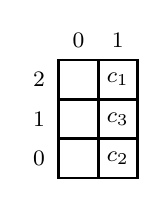
\begin{tikzpicture}[scale=0.5,inner sep=0.7mm]
        \foreach \y in {0,...,2} {
        \foreach \x in {0,...,1} {
                \draw [draw=black, line width=1pt] (\x,\y) rectangle (\x+1,\y+1);
        }
        }

        \node at (1.5,0.5){\footnotesize $c_{2}$};
        \node at (1.5,1.5){\footnotesize $c_{3}$};
        \node at (1.5,2.5){\footnotesize $c_{1}$};
        \foreach \x in {0,...,1} {
            \node at (\x+0.5,3.5){{\footnotesize $\x$}};
        }
        \foreach \y in {0,...,2} {
            \node at (-0.5,\y+0.5){{\footnotesize $\y$}};
        }

\end{tikzpicture}
}
\end{minipage}
\caption{TITRE A AJOUTER}
\label{fig:NOMFIGURE}
\end{center}
\end{figure}
